\documentclass[11pt,a4paper]{report}

%adjust your page margins here
\usepackage[top=1.0in, bottom=1.25in, left=1.5in,right=1.0in]{geometry} % setting the page alignment with this package
\usepackage[pdftex]{graphicx} %for embedding images
\usepackage[dvips, bookmarks,  colorlinks=false]{hyperref} %for creating links in the pdf version and other additional pdf attributes, no effect on the printed document
\hypersetup{%
    pdfborder = {0 0 0}
}
\usepackage[final]{pdfpages} %for embedding another pdf, remove if not required
\usepackage{float} %used for figure placement with H as a parameter
\usepackage{hyperref}
\usepackage{pslatex} % for times new roman, old package, but works
\usepackage{array} % for making text bold in table
\usepackage{setspace}
\usepackage{float}
\usepackage{enumerate}
\usepackage{longtable}
\usepackage{cite}
\usepackage{amsmath}
\begin{filecontents}{publications.bib}
@book{IntegratedDocumentClustering,
	title={Integrated Document Clustering and Multidocument Summerization},
	author={Dingding Wang, Shenghuo Zhu, Tao Li, Yun Chi and Yihong Gong},
	year={2011},
	publisher={ACM Transactions on Knowledge Discovey}
}
\end{filecontents}
\usepackage[font=small,labelfont=bf]{caption}
\def\figurename{\textbf{Figure }}

\usepackage{listings}
\usepackage{color}

\definecolor{dkgreen}{rgb}{0,0.6,0}
\definecolor{gray}{rgb}{0.5,0.5,0.5}
\definecolor{mauve}{rgb}{0.58,0,0.82}
 
\lstset{ %
  language=Java,                % the language of the code
  basicstyle=\footnotesize,           % the size of the fonts that are used for the code
  numbers=left,                   % where to put the line-numbers
  numberstyle=\tiny\color{gray},  % the style that is used for the line-numbers
  stepnumber=1,                   % each line is numbered
  numbersep=5pt,                  % how far the line-numbers are from the code
  backgroundcolor=\color{white},      % choose the background color. You must add \usepackage{color}
  showspaces=false,               % show spaces adding particular underscores
  showstringspaces=false,         % underline spaces within strings
  showtabs=false,                 % show tabs within strings adding particular underscores
  frame=single,                   % adds a frame around the code
  rulecolor=\color{black},        % if not set, the frame-color may be changed on line-breaks within not-black text (e.g. commens (green here))
  tabsize=2,                      % sets default tabsize to 2 spaces
  captionpos=b,                   % sets the caption-position to bottom
  breaklines=true,                % sets automatic line breaking
  breakatwhitespace=false,        % sets if automatic breaks should only happen at whitespace
  title=\lstname,                   % show the filename of files included with \lstinputlisting;
                                  % also try caption instead of title
  keywordstyle=\color{blue},          % keyword style
  commentstyle=\color{dkgreen},       % comment style
  stringstyle=\color{mauve},         % string literal style
  escapeinside={\%*}{*)},            % if you want to add a comment within your code
  morekeywords={*,...}               % if you want to add more keywords to the set
}

%For the header and footer
\usepackage{fancyhdr}
\fancypagestyle{plain}{%
\fancyfoot[L]{\emph{Department of Computer Science and Engineering, TKMCE, Kollam}} % except the center
\fancyfoot[R]{\thepage}
\renewcommand{\headrulewidth}{0.4pt}
\renewcommand{\footrulewidth}{0.4pt}
}

\pagestyle{fancy}

\rhead{\emph{Multi-Document Data Summarization}}

\fancyfoot[LO,LE]{\emph{Department of Computer Science and Engineering, TKMCE, Kollam}}
\cfoot{}
\fancyfoot[RO, RE]{\thepage}
\renewcommand{\headrulewidth}{0.4pt}
\renewcommand{\footrulewidth}{0.4pt}
%For the header and footer Over

%Page Border
\usepackage{pgf}
\usepackage{pgfpages}

\pgfpagesdeclarelayout{boxed}
{
  \edef\pgfpageoptionborder{0pt}
}
{
  \pgfpagesphysicalpageoptions
  {%
    logical pages=1,%
  }
  \pgfpageslogicalpageoptions{1}
  {
    %border code=\pgfsetlinewidth{0pt}\pgfstroke,%
    %border shrink=\pgfpageoptionborder,%
    %resized width=.95\pgfphysicalwidth,%
    %resized height=.95\pgfphysicalheight,%
    center=\pgfpoint{.5\pgfphysicalwidth}{.5\pgfphysicalheight}%
  }%
}
\pgfpagesuselayout{boxed}
\setlength{\parindent}{1cm}
%GLOBAL SETTINGS OVER, DOCUMENT BEGINS
\begin{document}
\renewcommand\bibname{References}
\lhead{ }

%FROM HERE YOUR PAGES START GETTING ADDED

% includes the cover page
\newpage
\begin{center}
\thispagestyle{empty}
\Large{\textbf{A PROJECT REPORT\\ \large{ON}}}\\[0.5cm]
\LARGE{\textsc {\textbf{``Multi-Document Data Summerization''}}}\\[0.5cm]
\vspace{0.3cm}
\Large{\textbf{\\Submitted to}}
\LARGE{\textbf{\\UNIVERSITY OF KERALA\\}}
\vspace{1cm}
\Large{\textbf{\\In Partial Fulfilment of the Requirement for the Award of\\}}
\Large{\textbf{\\BACHELOR'S DEGREE IN\\COMPUTER ENGINEERING}}
\vspace{0.5cm}
\Large{\textbf{\\BY}}\\[0.5cm]
\begin{table}[h]
\centering
\Large{
\begin{tabular}{>{\bfseries}lc>{\bfseries}r}
Abu Abraham & & 8101\\Arjun N & & 8106\\Balanarayanan & & 8107\\Clive Verghese & & 8110\\
\end{tabular}}
\end{table}
\vspace{0.5cm}
\large{\textbf{UNDER THE GUIDANCE OF}}\\
\large{\textbf{PROF. Ansamma John}}\\
\vspace{1cm}
\large{\textbf{DEPARTMENT OF COMPUTER SCIENCE AND ENGINEERING}}\\
\Large{\textbf{THANGAL KUNJU MUSLIAR COLLEGE OF ENGINEERING}}\\
\large{\textbf{KOLLAM, KERALA- PINCODE}}
\large{\textbf{\\2012-2013}}\\
\vspace{0.5cm}
\Large{\textbf{AFFILIATED TO\\}}
\LARGE{\textbf{UNIVERSITY OF KERALA}}
\newpage
\end{center}
\newpage

%\newpage
\begin{center}
\thispagestyle{empty}
\Large{\textbf{A PROJECT REPORT\\ON}}\\[0.2cm]
\Large{\textsc {\textbf{``MULTI-DOCUMENT DATA SUMMERIZATION''}}}\\
\Large{\textbf{\\Submitted to}}
\LARGE{\textbf{\\UNIVERSITY OF KERALA\\}}
\large{\textbf{\\In Partial Fulfilment of the Requirement for the Award of\\}}
\LARGE{\textbf{\\BACHELOR'S DEGREE IN\\COMPUTER SCIENCE AND ENGINEERING}}
\vspace{0.1cm}
\Large{\textbf{\\BY}}\\[0.2cm]
\begin{table}[h]
\centering
\Large{
\begin{tabular}{>{\bfseries}lc>{\bfseries}r}
Abu Abraham & & 8101\\Arjun N & & 8106\\Balanarayan & & 8108\\Clive Verghese & & 8110\\
\end{tabular}}
\end{table}
\large{\textbf{UNDER THE GUIDANCE OF}}\\
\large{\textbf{PROF. Ansamma John}}\\[0.5cm]

\includegraphics[scale=0.5]{project/images/jscoe_logo}\\
\large{\textbf{DEPARTMENT OF COMPUTER SCIENCE AND ENGINEERING}}\\
\Large{\textbf{THANGAL KUNJU MUSLIAR COLLEGE OF ENGINEERING}}\\
\large{\textbf{KOLLAM, KERALA - PINCODE}}
\large{\textbf{\\2012-2013}}\\[0.5cm]
\Large{\textbf{AFFILIATED TO}}\\[0.5cm]

\includegraphics[scale=3.0]{project/images/uop-logo}\\
\LARGE{\textbf{UNIVERSITY OF KERALA}}
\newpage

\end{center}
%\newpage

% includes the certificate page
%\begin{center}
\thispagestyle{empty}

\LARGE{\textbf{THANGAL KUNJU MUSLIAR COLLEGE OF ENGINEERING}} \\ 
\large{\textbf{Department of Computer Science and Engineering}}\\
\large{\textbf{Kollam, Kerala – PINCODE}}\\[0.5cm]


\includegraphics[scale=0.5]{project/images/jscoe_logo}\\[0.5cm]

{\Huge \textbf{CERTIFICATE}}\\[0.5cm]
\end{center}
\linespread{1.13}
\large{\centering{This is certify that the project entitled}\\[0.2cm]
\textbf{\Large{\centering{``Multi-Document Data Sumerization``}}}\\[0.2cm]
\centering{submitted by}\\[0.2cm]
\begin{table}[h]
\centering
\large{
\begin{tabular}{>{\bfseries}lc>{\bfseries}r}
Abu Abraham & & 8101\\Arjun N & & 8106\\Balanarayanan & & 8108\\Clive Verghese & & 8110\\
\end{tabular}}
\end{table}
 is a record of bonafide work carried out by them, in the partial
 fulfilment of the requirement for the award of Degree of Bachelor of
 Engineering (Computer Engineering) at NAME OF COLLEGE, Pune under the 
 University of Pune. This work is done
 during year 2012-2013, under our guidance.}\\[0.5cm]
\large{\textbf{Date:\hspace*{1.0cm}/\hspace*{1.0cm}/}}\\
\begin{spacing}{0}
\vspace{3.0cm}
\large{\textbf{(Prof. GUIDE NAME)}}\hspace*{1.2in}\large{\textbf{(Prof. PROJECT COORD NAME)}}\\
\hspace*{0.7in}\textbf{Project Guide}\hspace*{2.3in}\textbf{Project Coordinator}\\[3cm]
\hspace*{0.5cm}\large{\textbf{(Prof. HOD NAME)}}\hspace*{0.8in}\large{\textbf{(Dr. PRINCIPAL NAME)}}\\
\textbf{HOD, Computer Department}\hspace*{0.8in}\textbf{Principal}\hspace*{1.1in}\textbf{External Examiner}
\end{spacing} 
%\newpage

% includes the acknowledgements page
\begin{center}
\thispagestyle{empty}
\LARGE{\textbf{Acknowledgements}}\\[1cm]
\end{center}
\linespread{1.13}
\large{\paragraph{}We are profoundly grateful to \textbf{Prof. Anasamma John} for her expert guidance
and continuous encouragement throughout to see that this project rights its
target since its commencement to its completion.}
\large{\paragraph{}We would like to express deepest appreciation towards \textbf{Dr. Chitraprasad D}, 
Head of Department of Computer Science and Engineering and \textbf{Dr. Amar Nishad}, Project Coordinator whose
invaluable guidance supported us in completing this project.}
\large{\paragraph{}At last we must express our sincere heartfelt gratitude to all the staff members
of Computer Engineering Department who helped us directly or indirectly during this course of work.}
\begin{flushright}
{
Abu Abraham\\
Arjun N\\
Balanarayanan\\
Clive Verghese
}
\end{flushright}
\newpage
 
\newpage

%\begin{center}
\thispagestyle{empty}
\vspace{2cm}
\LARGE{\textbf{ABSTRACT}}\\[1.0cm]
\end{center}
\thispagestyle{empty}
\large{\paragraph{}Your abstract, paragraph 1.}
\large{\paragraph{}Your abstract, paragraph 2.}\\
\textbf{Keywords: }keyword1, keyword2 % adds the Research Methodology page
%\newpage

%TABLE OF CONTENTS AND LIST OF FIGURES ARE AUTOMATICALLY ADDED BY FOLLOWING COMMANDS
%ADD FIGURE OF TABLES IF YOU NEED TO, CHECK DOCUMENTATION
\pagenumbering{roman} %numbering before main content starts


%To reset the Header & Footer for TOC and LOF
\pagestyle{empty}
\addtocontents{toc}{\protect\thispagestyle{empty}}
\tableofcontents % adds Index Page

%\addtocontents{lof}{\protect\thispagestyle{empty}}
%\listoffigures % adds List of Figures
%\cleardoublepage

%And reset back the settings we choose for Header and Footer
\pagestyle{fancy}

\newpage
\pagenumbering{arabic} %reset numbering to normal for the main content
\chapter{Introduction}

\section{General Introduction}
\paragraph{}Summarization is the process of reducing a text document into a document of smaller size that retains the most important points of the original document. Automatic summarization techniques such as extraction and abstraction provide efficient methods for the creation of document summaries.

\paragraph{}Multi-document summarization technique is an extension to this ,in the sense Multi-document Summarization is an automatic procedure aimed at extraction of information from multiple texts written about the same topic. It creates information reports that are both concise and comprehensive. With different opinions being put together \& outlined, every topic is described from multiple perspectives within a single document. While the goal of a brief summary is to simplify information search and cut the time by pointing to the most relevant source documents, comprehensive multi-document summary should itself contain the required information, hence limiting the need for accessing original files to cases when refinement is required. Automatic summaries present information extracted from multiple sources algorithmically, without any editorial touch or subjective human intervention, thus making it completely unbiased.
 
\paragraph{}Document clustering and multi-document summarization have definitely emerged as the two fundamental tools for understanding document data and have attracted much attention in recent years. Given a collection of documents, document clustering aims to partition them into different groups called clusters; so that the documents in the same group are similar to each other, while the documents in different clusters are dissimilar .Multi-document summarization is an effective way to summarize each document cluster. In general, there are two types of summarization: extractive summarization and abstractive summarization. Extractive summarization selects the important sentences from the original documents to form a summary, while abstractive summarization paraphrases the corpus using novel sentences. So, extractive summarization usually ranks the sentences in the documents according to their scores calculated by a set of pre defined features, such as term frequency-inverse sentence frequency, sentence or term position and number of keywords.

\paragraph{}Consider the situation where the user issues a search query, for instance on a news topic, and the retrieval system finds hundreds of closely-ranked documents in response. Many of these documents are likely to repeat much the same information, while differing in certain parts. Summaries of the individual documents would help, but are likely to be very similar to each other, unless the summarization system takes into account other summaries that have already been generated.


\paragraph{}
\begin{itemize}
\item The degree of redundancy in information contained within a group of topically-related articles is much higher than the degree of redundancy within an article, as each article is apt to describe the main point as well as necessary shared background. Hence anti-redundancy methods are more crucial.
\item A group of articles may contain a temporal dimension, typical in a stream of news reports about an unfolding event. Here later information may over- ride earlier more tentative or incomplete accounts
\item The compression ratio (i.e. the size of the summary with respect to the size of the document set) will typically be much smaller for collections of dozens or hundreds of topically related documents than for single document summaries. Summarization becomes significantly more difficult when compression demands increase.
\item The co-reference problem in summarization presents even greater challenges for multi- document than for single-document summarization.\cite{Publication2}
\end{itemize}
\section{Motivation}
\paragraph{} In today’s world there are multiple sources giving us the same information. Like news websites, online reference websites, book and movie reviews etc. It is simply impossible and not practically easy to read information from everywhere. So there’s a need to deliver consolidated and summarized information to a user.
\paragraph{} We ourselves have often encountered this problem. For looking up for writing reports and assignments we find that most information from various sources are same or redundant, given the same topic but each article can contain a line or information that is not present in all others . So we have to include that as well along with the redundant information.
\paragraph{} So the perfect tool to tackle this problem was a multi document summarizer. In this age of information explosion, the scope for a multi document summarizer is huge. This was the motivation we had for taking up this project. 
\paragraph{} With the inclusion of a document fetcher and classifier that automatically fetches documents from the web mainly news articles our project became more real world and useable for the common man. We also would like to provide a web interface that shows the trending stories of the hour. Hence a user can look at the concise and relevant information about the top stories that are trending at the hour.

\section{Problem Definition}
\paragraph{} The problem of data summarization is an qualitative one rather than a quantitative one .It focuses on creating on reading human readable summery of given document or documents.
\paragraph{} The Task set of our project includes Fetching the news articles from the web automatically, Cluster it using a naive algorithm and generating summaries of each cluster based on headlines or topics.
\paragraph{} Initial steps can easily be implemented using the help of a parser library like Beautiful Soup\cite{BeautifulSoup}. For the clustering we use a naïve algorithm like hierarchical clustering \cite{HClustering}. The heart of the project is the Multi-Document Summarizer. The summarizer can be subdivided into five parts.
\begin{enumerate}[1. ]
 \item Sentence Extraction
 \item Topic Detection
 \item Information Extraction
 \item Sentence Extraction
 \item Sentence Ordering
\end{enumerate}
	
\paragraph{} The steps we focus are Extraction and Ordering. Others are beyond the scope of this project and too complex to implement as it involves breaking down of sentences into parts of speech etc.

\paragraph{} Finally we generate a web page which shows the summaries of hot news topics we fetched and created summaries of. Overall the problem is a multi faceted one and resembles a real world one. From the python back end to the HTML front end.
 % adds the introduction page
\section{Literature Review} 
\paragraph{} With rapid growth of internet and the upcoming of internet services since 1995 ,the amount of data and information being shared and accessed  throughout the world has increased rapidly. An efficient method to improve the viewablity and accessibility of documents was required and Multi-document Summarization emerged as one the main tool. Research in this field was started back then and none of the designed algorithms could satisfy the entire requirements, each had shortcoming in certain fields. Hence a proper combination of various Algorithms was required to obtain a decent result and we have implemented ours in that way. 
 
\paragraph{} A straightforward approach in Multi-document Summarization is to first cluster the documents and then summarize each document cluster using summarization methods. However, most of the current summarization methods are solely based on the sentence-term matrix and ignore the context dependence of the sentences. As a result, the generated summaries lack guidance from the document clusters. Dingding Wang    proposed a new language model to simultaneously cluster and summarize documents by making use of both the document-term and sentence- term matrices. By utilizing the mutual influence of document clustering and summarization, his method makes a better document clustering method with more meaningful interpretation and an effective document summarization method with guidance from document clustering .  
 
\paragraph{} Traditional clustering techniques such as hierarchical and partitioning methods have been used in clustering documents. Hierarchical clustering proceeds successively by building a tree of clusters using bottom-up or top-down approaches. For example, hierarchical agglomerative clustering (HAC) \cite{Duda} is a typical bottom-up hierarchical clustering method, which takes each document as a singleton cluster to start off with and then merges pairs of clusters until all clusters have been encapsulated into one final cluster that contains all documents. Partitioning methods attempt to directly decompose the docu-ment collection into a number of disjoint classes such that the documents in a cluster are more similar to one another than the documents in other clusters \cite{HeEtAl}. For example, K-means \cite{Duda} is a typical partitioning method, which aims to minimize the sum of the squared distances between the documents and the corresponding cluster centers. 
 
\paragraph{} A  paper by Jade Goldstein\cite{Publication2} discusses a text extraction approach to multi-document summarization that builds on single-document summarization methods by using additional, available information about the document set as a whole and the relationships between the documents. His approach addresses these issues by using domain independent techniques based mainly on fast, statistical processing, a metric for reducing redundancy and maximizing diversity in the selected passages, and a modular framework to allow easy parameterization for different genres, corpora characteristics and user requirements.
 
\paragraph{} Ordering information is difficult but an important task for application generating natural language texts such as multi-document summarization. In Multi-doument Summarization information is selected from a set of source documents.Therefore the optimal ordering of those selected pieces of information to create coherent summary is not obvious.To capure the preference of a sentence againts another sentence, 5 prefernce experets were intoduced by Danushka Bollegala  chronology, probablistic, topical-closeness, precedence and succession.The proposed sentence ordering algorithm considers pairwise comparison between sentences to determine a total ordering , using a greedy algorithm, thereby avoiding the combinatorial time complexity typically associated wih total ordering task. 
 
 \paragraph{} A preference learning approach to sentence ordering for multi - document summarization
\chapter{Terms And Defination}
\begin{itemize}
\item \textbf{Document} \newline A piece of electronic text matter that provides information or evidence or that serves as an official record.

\item \textbf{Summarization} \newline The act of preparing summary of electronic text document;

\item \textbf{Stop words} \newline Stop words are words which are filtered out prior to, or after, processing of natural language data (text)

\item \textbf{Tokenization} \newline Tokenization is the process of breaking a stream of text up into words, phrases, symbols, or other meaningful elements called tokens. The list of tokens becomes input for further processing such as parsing or text mining. Tokenization is useful both in linguistics (where it is a form of text segmentation), and in computer science, where it forms part of lexical analysis. The tokenize module provides a lexical scanner for Python source code, implemented in Python. 

\item \textbf{Stemming} \newline Stemming is the process for reducing inflected (or sometimes derived) words to their stem, base or root form—generally a written word form. The stem need not be identical to the morphological root of the word. There are several types of stemming algorithms which differ in respect to performance and accuracy and how certain stemming obstacles are overcome. e.g : \textbf{Lookup algorithms}
\paragraph{} A simple stemmer looks up the inflected form in a lookup table. The advantages of this approach are that it is simple, fast, and easily handles exceptions. The disadvantages are that all inflected forms must be explicitly listed in the table: new or unfamiliar words are not handled, even if they are perfectly regular (e.g. iPads ~ iPad), and the table may be large. For languages with simple morphology, like English, table sizes are modest, but highly inflected languages like Turkish may have hundreds of potential inflected forms for each root.A lookup approach may use preliminary part-of-speech tagging to avoid over stemming. 
\item \textbf{Vector} \newline
Each sentence is represented as n-Dimensional spatial coordinate. Each word in a sentence is represented as vector. Though if a sentence contain n words it would represent n dimensional vector in space. Its relevance is calculated using cosine law  

\item \textbf{Clustering} \newline
Clustering is the task of grouping a set of objects in such a way that objects in the same group (called cluster) are more similar (in some sense or another) to each other than to those in other groups (clusters). It is a main task of exploratory data mining, and a common technique for statistical data analysis used in many fields, including machine learning, pattern recognition, image analysis, information retrieval, and bioinformatics. There are several clustering methods are available,  method we adopted here is hierarchical clustering.

\item \textbf{Hierarchical clustering} \newline
Is a method of cluster analysis which seeks to build a hierarchy of clusters. Strategies for hierarchical clustering generally fall into two types:
\begin{enumerate}[a. ]
\item \textbf{Agglomerative :}  This is a "bottom up" approach: each observation starts in its own cluster, and pairs of clusters are merged as one moves up the hierarchy.
\item \textbf{Divisive :} This is a "top down" approach: all observations start in one cluster, and splits are performed recursively as one moves down the hierarchy.
\end{enumerate}

\item \textbf{Cosine Similarity} \newline
Cosine similarity is a measure of similarity between two vectors of an inner product space that measures the cosine of the angle between them. The cosine of 0° is 1, and it is less than 1 for any other angle. It is thus a judgement of orientation and not magnitude: two vectors with the same orientation have a Cosine similarity of 1, two vectors at 90° have a similarity of 0, and two vectors diametrically opposed have a similarity of -1, independent of their magnitude. Cosine similarity is particularly used in positive space, where the outcome is neatly bounded in [0,1].Note that these bounds apply for any number of dimensions, and Cosine similarity is most commonly used in high-dimensional positive spaces. For example, in Information Retrieval, each term is notionally assigned a different dimension and a document is characterized by a vector where the value of each dimension corresponds to the number of times that term appears in the document. Cosine similarity then gives a useful measure of how similar two documents are likely to be in terms of their subject matter.

\item \textbf{Sentence} \newline
A set of words that is complete in itself, typically containing a subject and predicate, conveying a statement, question, exclamation.

\item \textbf{Corpus} \newline
Collection of data set.


\item \textbf{Chronological Expert} \newline
Chronological expert reflects the chronological ordering by returning 0 or 1 or 0.5 while comparing 2 sentences in their chronological order. if both sentence have same chronological preference, returns 0.5. Other wise 1 or zero depending on the priority.

\item \textbf{Precedence Expert} \newline
We define the precedence, pre(I),of a sentence as follows,
\begin{center}
\begin{equation}
pre(I) = \frac{1}{|Q|}\sum_{q \in Q, p \in Pq}^{N} maxism(p,I)
\end{equation}
\end{center}
here Pq is the set of sentences preceding the sentence q $\in$ Q, the original document,and $|Q|$ denotes the total number of sentence that we have ordered so far. We calculate sim(p,I) using cosine similarity. The formalism of precedence proposed in the equation above captures the idea of similarity between preceding information of a sentence in an original document and an extracted sentence that must be ordered in the summary. Consequently we consider all the sentence in the Q. The preference function returns 0 or 1 or 0.5 according to their similarity factor.
\item \textbf{Succession Expert} \newline
\begin{center}
\begin{equation}
succ(I) = \frac{1}{|Q|}\sum_{q \in Q, p \in Pq}^{N} maxism(s,I)
\end{equation}
\end{center}
Here, We calculate sim(s,I) using cosine similarity.Sq is the set of sentences that appear after(succeeds) the sentence q in the original document from which q was extracted. Succession score compares each sentence that appear in Sq against the sentence I that we must order next. if some sentence in Sq contains information similar to that conveyed by I, the I obtains a higher succession score. Because it is sufficient that at least one sentence similar to I in each Succeeding block, we consider the maximum similarity. Moreover, we divide the sum of similarity scores by the total number of sentences in Q to avoid any bias toward longer Q segments. Succession expert return 0 or 1 or 0.5 according to their succession similarity factor.

\item \textbf{Converge} \newline
Come together from different directions so as eventually to meet.

\item \textbf{Redundancy} \newline
Duplication of same sentences in summary containing same meaning
\item \textbf{TF-IDF} \newline
Tf–idf, term frequency–inverse document frequency, is a numerical statistic which reflects how important a word is to a document in a collection or corpus. It is often used as a weighting factor in information retrieval and text mining. The tf-idf value increases proportionally to the number of times a word appears in the document, but is offset by the frequency of the word in the corpus, which helps to control for the fact that some words are generally more common than others.
\paragraph{} Variations of the tf-idf weighting scheme are often used by search engines as a central tool in scoring and ranking a document's relevance given a user query. tf-idf can be successfully used for stop-words filtering in various subject fields including text summarization and classification. One of the simplest ranking functions is computed by summing the tf–idf for each query term; many more sophisticated ranking functions are variants of this simple model.

\item \textbf{JSON} \newline
The JSON format is often used for serializing and transmitting structured data over a network connection. It is used primarily to transmit data between a server and web application, serving as an alternative to XML.
\item \textbf{XML} \newline
Extensible Markup Language (XML) is a markup language that defines a set of rules for encoding documents in a format that is both human-readable  and machine-readable. The design goals of XML emphasize simplicity, generality, and usability over the Internet.  It is a textual data format with strong support via Unicode for the languages of the world. Although the design of XML focuses on documents, it is widely used for the representation of arbitrary data structures, for example in web services. 
\item \textbf{HTML} \newline
Hyper Text Markup Language (HTML) is the main markup language for creating web pages and other information that can be displayed in a web browser.HTML elements form the building blocks of all websites. HTML allows images and objects  to be embedded and can be used to create interactive forms. It provides a means to create structured documents by denoting structural semantics for text such as headings, paragraphs, lists, links, quotes and other items. It can embed scripts written in languages such as JavaScript which affect the behavior of HTML web pages.


\end{itemize}
\chapter{Materials and Methodology}
\section{System Design}
\paragraph{} The system deals with fetching, summarization and creation of front end results for the user. We have used extensive use of python libraries to aid us in parsing data from RSS feeds and extracting data from websites. 
\paragraph{} Next stage was to cluster the documents fetched based on the topics. So we're able to generate input documents for the summarizer. The summarizer using the below mentioned algorithms and methods generate a summery based on length specified. Finally a JSON file is generated for the generated summaries. 
\paragraph{} An HTML front end using AJAX is used to fetch this JSON file to the user. The block diagram given below will make the whole procedure clearer.
\newpage
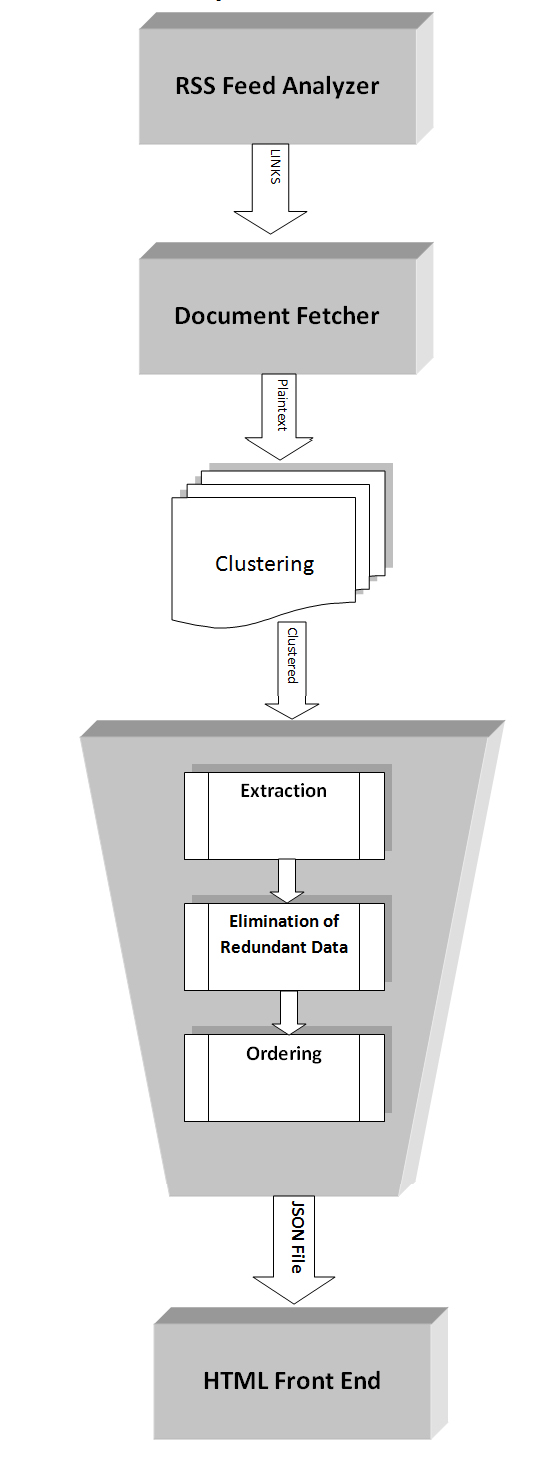
\includegraphics[scale=0.4]{my/images/gh}
\subsection{RSS Feed Analyzer}
\paragraph{} Really Simple Syndication (RSS) is a family of web feed formats used to publish frequently updated works—such as blog entries, news headlines, audio, and video—in a standardized format. It is universally used by news websites for providing news headlines and links to clients. We use a python library developed by Leonard Richardson knows as BeautifulSoup\cite{BeautifulSoup}. It is used to extract tags from the feed page.
\begin{lstlisting}
<xml version="1.0" encoding="UTF-8" >
<rss version="2.0">
<channel>
 <title>RSS Title</title>
 <description>This is an example of an RSS feed</description>
 <link>http://www.someexamplerssdomain.com/main.html</link>
 <lastBuildDate>Mon, 06 Sep 2010 00:01:00 +0000 </lastBuildDate>
 <pubDate>Mon, 06 Sep 2009 16:45:00 +0000 </pubDate>
 <ttl>1800</ttl>
 
 <item>
  <title>Example entry</title>
  <description>Here is some text containing an interesting description.</description>
  <link>http://www.wikipedia.org/</link>
  <guid>unique string per item</guid>
  <pubDate>Mon, 06 Sep 2009 16:45:00 +0000 </pubDate>
 </item>
\end{lstlisting}
\subsection{Document Fetcher}
\paragraph{}Document fetcher is used for fetching articles from the links in the RSS feeds obtained in the above step. Here also we use the above mentioned library BeautifulSoup\cite{BeautifulSoup}. We designed individual fetchers for each site since the HTML framework of each site is different from each other. This was a relatively tiresome task to do.
\paragraph{}	Document Fetcher takes in input as links and gives output as the documents or articles in those links and headings in plain text format. This can be fed into the summarizer as input.
\subsection{Clustering}
\paragraph{} Clustering is used to group large number of documents into clusters. We require this since there would be different news articles fetched from the web and we need to cluster them and group them for generating summery for a group of documents.
\paragraph{}	There are various clustering algorithms available .Old ones include centroid clustering and naïve similarity algorithms. We use the concept of Hierarchical Clustering. Hierarchical clustering is a method of cluster analysis which seeks to build a hierarchy of clusters. Strategies for hierarchical clustering generally fall into two types:
\begin{enumerate}[a. ]
\item \textbf{Agglomerative :} This is a "bottom up" approach: each observation starts in its own cluster, and pairs of clusters are merged as one moves up the hierarchy.
\item \textbf{Divisive :} This is a "top down" approach: all observations start in one cluster, and splits are performed recursively as one moves down the hierarchy.
\end{enumerate}
\begin{equation}
similarity = \cos{\theta} = \frac{A.B}{\|A\|.\|B\|}
\end{equation}
\paragraph{}The choice of an appropriate metric will influence the shape of the clusters, as some elements may be close to one another according to one distance and farther away according to another. We used Cosine Similarity for determining the clusters.
\subsection{Summarization}
\paragraph{} The heart of the project is called the summarizer. This takes in multiple documents and generates the summery based on the given parameters. Multi-document summarization tackles the information overload problem by providing a condensed and coherent version of a set of documents. Among a number of sub-tasks involved in multi-document summarization including sentence extraction, topic detection, sentence ordering, information extraction, and sentence generation, most multi-document summarization systems have been based on an extraction method, which identifies important textual segments (e.g. sentences or paragraphs) in source documents
\subsubsection{Sentense Extraction}
\paragraph{} Sentence extraction is the process of retrieving relevant and non redundant sentences from the document set. We used various methods for implementing this like Cosine Ranking, Centroid Method, and finally the clustering method. In out tests we found out that first method the Cosine Ranking was not very efficient in many cases and was abandoned.
\paragraph{}	The method we use mainly is known as the Centroid method. In this method one aims to create a Centroid of sentences by repeatedly removing the ones with low similarity with the sentence in Centroid and also the ones which have high similarity since they are redundant .This ensures that we get a good set of sentences which are relevant and non redundant.
\begin{lstlisting}
while (n<N)
	for each sentence in documents:
		Find cosine similarity with document vector;
		if( cs  > threshold 1)
			Add sentence to set
		if(cs < threshold2)
			Remove sentence from document 
		n++
	end  for
end while
\end{lstlisting}
\paragraph{} The method that improves the extraction process even more is known as Clustering combined with Centroid .This ensures even better result and more relevant sentences are selected due the initial clustering operation. This is basically grouping a set of objects in such a way that objects in the same group (called cluster) are more similar (in some sense or another) to each other than to those in other groups (clusters)
\subsubsection{Ordering}
\paragraph{} The next important thing to after extraction of sentences is that it needs to be ordered properly so that the user feels continuity while reading. This makes it one of the most complex steps in summarization as a whole since there’s no quantitative way to check the validity of this operation. We can only rely on human verification for this. A summary with improperly ordered sentences both confuses the reader and degrades the quality/reliability of the summary. Study shows that the proper order of extracted sentences significantly improves their readability. It has been experimentally shown that the time taken to read a summary strongly correlates with the arrangement of sentences in the summary.
\paragraph{}	But despite this some probabilistic and chronological methods exist for doing this. We employ 3 such methods here. They are 1) Chronological 2) Precedence 3) Succession. We use these three methods to find the relative rank of a sentence in the summary. Each of this are assigned weights that when varied will produce different weights for each method.
\begin{enumerate}[a. ]
\item \textbf{Chronological Expert :} \newline The author of a particular document is likely to order the sentences logically to make the document coherent. Therefore, for sentences belonging to a particular document, we can safely retain this original order given by the author. In single document summarization this simple ordering strategy is often adequate to order all the extracted sentences because those sentences belong to a single document.

Chronological ordering we use can be summarized by the function 
\begin{equation}
PREF_{chro}(u,v,Q) = \begin{cases}
	1 & T(u) < T(v)\\
	1 & [D(u) = D(v)] \wedge [N(u) < N(v)]\\
	0.5 & [T(u) = T(v)] \wedge [D(u) \neq D(v)]\\
	0 & otherwise
\end{cases} 
\end{equation}
\paragraph{} In the above equation the expert returns 1 if the relative position of the first 	sentence is in front of the second and they both are in the same document. It does the 		same if they are from different documents .It returns the value 0.5 if they both are in 	same position in the document.
\item \textbf{Precedence expert :} In extractive multi-document summarization, only the important sentences that convey the main points discussed in source documents are selected to be included in the summary. However, a selected sentence can presuppose information from other sentences that were not selected by the sentence extraction algorithm.
\begin{equation}
pre(I) = \frac{1}{|Q|}\sum_{q \in Q, p \in Pq}^{N} maxism(p,I)
\end{equation}
\paragraph{} Here the precedence value of a sentence is calculated by taking the maximum cosine similarity of obtained when cosine similarity is calculated for n sentences before that. Finally when two sentences are compared this relation is used.
\begin{equation}
PREF_{pre}(u,v,Q) = \begin{cases}
	0.5 & [Q \neq \emptyset ] \vee [pre(u) = pre(v)]\\
	1 & [Q \neq \emptyset ] \wedge [pre(u) > pre(v)]\\
	0 & otherwise
\end{cases}
\end{equation}
\item \textbf{Succession Expert :} In extractive multi-document summarization, sentences that 	describe a particular event are extracted from a set of source articles.
\begin{equation}
PREF_{succ}(u,v,Q) = \begin{cases}
	0.5 & [Q \neq \emptyset ] \vee [succ(u) = succ(v)]\\
	1 & [Q \neq \emptyset ] \wedge [succ(u) > succ(v)]\\
	0 & otherwise
\end{cases}
\end{equation}
\item Usually, there exists a logical sequence among the information conveyed in the extracted sentences.
\begin{equation}
succ(I) = \frac{1}{|Q|}\sum_{q \in Q, p \in Pq}^{N} maxism(s,I)
\end{equation}
\paragraph{} Here the succession value of a sentence is calculated by taking the 			maximum cosine similarity of obtained when cosine similarity is calculated for n 	sentences after that. Finally when two sentences are compared this relation is used.
\begin{equation}
PREF_{succ}(u,v,Q) = \begin{cases}
	0.5 & [Q \neq \emptyset ] \vee [succ(u) = succ(v)]\\
	1 & [Q \neq \emptyset ] \wedge [succ(u) > succ(v)]\\
	0 & otherwise
\end{cases}
\end{equation}

\end{enumerate}
\subsubsection{Ordering Algorithm}
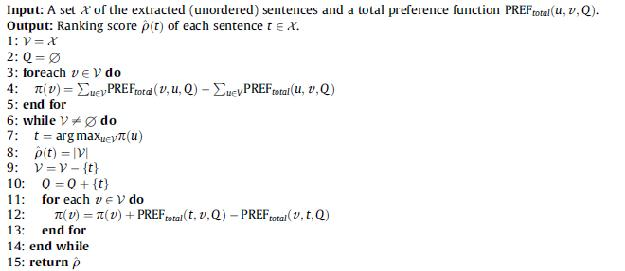
\includegraphics[scale=0.75]{my/images/algorithm}
\paragraph{} Algorithm greedily calculates the most eligible sentence for selection based on the combined effect of these three factors. The sentence so selected is removed from the summary set and the weights / potentials is updated for each vertex to reflect the removal of the sentence. This is repeated for all sentences in the selected set .  


\section{Platform Details}
\subsection{Python}

\paragraph{} Python is a general purpose, high-level programming language whose design philosophy emphasizes code readability. Python's syntax allows programmers to express concepts in fewer lines of code than would be possible in languages such as C and the language provides constructs intended to enable clear programs on both a small and large scale. Python is a programming language that lets you work more quickly and integrate your systems more effectively. Python has small and has clean source codes. Standard library is full of useful modules.
\paragraph{} Python supports multiple programming paradigms, including object-oriented, imperative and functional programming styles. It features a dynamic type system and automatic memory management and has a large and comprehensive standard library.
\paragraph{} Like other dynamic languages, Python is often used as a scripting language, but is also used in a wide range of non-scripting contexts. Using third-party tools, Python code can be packaged into standalone executable programs. Python interpreters are available for many operating systems.
\textbf{Syntax and Semantics}
\paragraph{} The syntax of the Python programming language is the set of rules that defines how a Python program will be written and interpreted (by both the runtime system and by human readers). Python was designed to be a highly readable language. It has a relatively uncluttered visual layout and uses English keywords frequently where other languages use punctuation. Python aims towards simplicity and generality in the design of its syntax.
\paragraph{} Python uses whitespace indentation, rather than curly braces or keywords, to delimit blocks; a feature also termed the off-side rule. An increase in indentation comes after certain statements; a decrease in indentation signifies the end of the current block.
\textbf{Features of Python}
\begin{enumerate}[1. ]
\item \textbf {Simple} \newline Python is a simple and minimalistic language. Reading a good Python program feels like reading English, although very strict English! This pseudo-code nature of Python is one of its greatest strengths.

\item \textbf{Easy to Learn} \newline As we will discover in this book, Python is very easy to get started with and has an extraordinarily simple syntax.
\item \textbf{Free and Open Source} \newline Python is an example of an open source software. In simple terms, you can freely distribute copies of the software, read the source code, make changes to it and use pieces of it in new free programs. Open source is based on the concept of a community which shares knowledge. This is one of the reasons why Python is so good - it is constantly improved by a community which just wants to see a better Python.
\item \textbf{High-level Language} \newline When you write programs in Python, you do not need to bother about low-level details such as managing the memory used by your program, etc.
\item \textbf{Portable} \newline Due to its open source nature, Python has been ported to (i.e. changed to make it work on) many platforms. All your Python programs can work on any of these platforms without requiring any changes as long as you are careful to avoid any system-specific features.
\item \textbf{Interpreted} \newline Python, on the other hand, does not need the compilation and linking/loading steps. You just run the program directly from source code. Internally, Python converts the source program into an intermediate form called bytecodes and then translates this into the native language of your specific system and then runs it. All this actually makes Python much easier to use since you do not have to worry about compiling the program, making sure the proper libraries are linked and loaded, etc. This also makes your Python programs more portable since you can just copy the program to another computer and it just works!
\item \textbf{Object Oriented} \newline Python supports both procedure-oriented programming as well as object-oriented programming. In procedure-oriented programming, the program is built around procedures or functions which are just reusable pieces of programs to which data is fed. In object-oriented programming, the program is built around objects which combine both data and functionality.


\item \textbf{Extensible} \newline If you need a critical piece of code in your program to run very fast or want to have a piece of algorithm to be hidden from the outside world, then you can write that part of the program in languages like C or C++ and then use that part from your Python programs.
\item \textbf{Embeddable} \newline You can embed Python in your programs written in other languages like C or C++ to give 'scripting' capabilities for your program's users.
\item \textbf{Extensive Libraries}
\end{enumerate}
\subsection{NLTK}
\paragraph{} The Python Standard Library is huge. It can help you with regular expressions, documentation generation, unit testing, threading, databases, web browsers, CGI, FTP, email, XML, HTML, WAV files, cryptography, GUI using Tk, and  many other system-specific functionality as well.
\paragraph{} NLTK is a leading platform for building Python programs to work with human language data. It provides easy-to-use interfaces to over 50 corpora and lexical resources such as WordNet, along with a suite of text processing libraries for classification, tokenization, stemming, tagging, parsing, and semantic reasoning.
\paragraph{} Thanks to a hands-on guide introducing programming fundamentals alongside topics in computational linguistics, NLTK is suitable for linguists, engineers, students, educators, researchers, and industry users alike. NLTK is available for Windows, Mac OS X, and Linux. Best of all, NLTK is a free, open source, community-driven project. 
\paragraph{} NLTK has been called “a wonderful tool for teaching, and working in, computational linguistics using Python,” and “an amazing library to play with natural language.”
\paragraph{} Natural Language Processing with Python provides a practical introduction to programming for language processing. Written by the creators of NLTK, it guides the reader through the fundamentals of writing Python programs, working with corpora, categorizing text, analyzing linguistic structure, and more.

\begin{enumerate}[1. ]
\item \textbf{NLTK Stemmers} \newline Interfaces used to remove morphological affixes from words, leaving only the word stem. Stemming algorithms aim to remove those affixes required for eg. grammatical role, tense, derivational morphology leaving only the stem of the word. This is a difficult problem due to irregular words (eg. common verbs in English), complicated morphological rules, and part-of-speech and sense ambiguities (eg. ceil- is not the stem of ceiling).
\item \textbf{NLTK Tokenizer Package} \newline Tokenizers divide strings into lists of substrings. For example, tokenizers can be used to find the list of sentences or words in a string. NLTK tokenizers can produce token-spans, represented as tuples of integers having the same semantics as string slices, to support efficient comparison of tokenizers. (These methods are implemented as generators.)
\item \textbf{NLTK Taggers} \newline This package contains classes and interfaces for part-of-speech tagging, or simply “tagging”. A “tag” is a case-sensitive string that specifies some property of a token, such as its part of speech. Tagged tokens are encoded as tuples (tag, token). This package defines several taggers, which take a token list (typically a sentence), assign a tag to each token, and return the resulting list of tagged tokens. Most of the taggers are built automatically based on a training corpus
\item \textbf{Corpus} \newline A large corpus can provide a wide variety of useful information, provided that there are decent tools to extract it. In Natural Language Processing (NLP), for example, statistical information obtained from large corpora (consisting of tens of millions of words) is used to inform many different tasks, ranging from guessing the most likely parsing for a sentence to determining the likelihood that a document matches key terms in a search.
\end{enumerate}
\paragraph{} NLTK has been used successfully as a teaching tool, as an individual study tool, and as a platform for prototyping and building research systems.
\subsection{SciPy-Cluster}
\paragraph{}This library provides Python functions for agglomerative clustering. Its features include  
generating hierarchical clusters from distance matrices 
computing distance matrices from observation vectors 
computing statistics on clusters 
cutting linkages to generate flat clusters 
\subsection{NumPy}
\paragraph{} NumPy is an extension to the Python programming language, adding support for large, multi-dimensional arrays and matrices, along with a large library of high-level mathematical functions to operate on these arrays. The ancestor of NumPy, Numeric, was originally created by Jim Hugunin with contributions from several other developers. In 2005, Travis Oliphant created NumPy by incorporating features of Numarray into Numeric with extensive modifications. NumPy is open source and has many contributors.



    
\chapter{Result And Analysis}
\paragraph{}	We evaluated our algorithms using mainly articles from News websites. They are mostly articles of small size and very similar in terms of content similarity. This generated summaries of fair quality and good readability. We also tried a few test cases with standard articles of greater length .But the results were not as good as the initial ones and showed improvements on various parameters like weights assigned to the ordering experts.
\paragraph{}	Results and analysis can mainly be divided into results of the three major steps we do. The initial clustering of documents, sentence extraction and sentence ordering. These three can be individually evaluated and finally contributes to the quality of the whole document.


\textbf{Document Clustering}
\paragraph{}	For creating an efficient clustering mechanism we varied the threshold value from .5 to 1.5 and while setting threshold as 1 a more precise output was obtained. Various methods were carried out starting with Euclidian distance method, tested with each parameter-single, average and complete. This approach was not found to be efficient and we moved on to the cosine method which had same parameters and keeping the parameter as ‘single’ gave the best result compared to the others. So after few trials we decided to use single as out primary method for this part of the problem.
\paragraph{}	Another question before us was to choose between Agglomerative or Divisive technique in hierarchical clustering. Here since due to the popularity of the method and ease of use we chose Agglomerative technique for clustering. Another problem we encountered during clustering was that articles like topics related to health care and an accident being clustered together. This was avoided by changing the parameters values.


\textbf{Sentence Extraction} 
\paragraph{}	Sentence extraction is done with Centroid method. Here we use two parameters to remove the similar ones and ones which have no similarity with the document. Adjusting this parameters can directly affect the overall number of sentences and also the relative relation between sentence and the whole document.
\paragraph{}	The threshold value for upper limit for eliminating redundancy is initialized with 0.9 and the lower limit for removing sentences of no relevance is 0.1. This value keeps on changing throughout the iteration till number of sentences to be selected or till convergence is reached.

	
Sentence Ordering
\paragraph{}	Ordering is one of the most difficult tasks in this to do and evaluate. In our work we first used a naïve algorithm using the sentence weight .This was somewhat accurate but decreased the readability of the summary since no importance was given to the original ordering
\paragraph{}	Next we tried to sort the ordered sentence based on the relative position of the sentence in the original document. This provided an even better result and increased the readability of the summary. Since original ordering was preserved it worked perfectly in articles of small lengths. But when the length of the input documents increased the ordering began to go wrong.
\paragraph{}	In the third stage we included the three ordering experts. viz Chronological, Precedence and Succession. Details of each have been explained in the system design. While calculating the rank of a sentence we use all these three combined. So weights have to be assigned to each expert
\paragraph{}	In our testing we found out that chronological expert was most important and gave it the most priority. Succession and precedence priorities were initially given same but on finer examination we found out that precedence should have been given more priority than precedence so finally the weights for each expert was as follows.
\begin{itemize}
\item Chronological, 0.5
\item Precedence, 0.3
\item Sucession, 0.2
\end{itemize}
\paragraph{} Sentences ordered with this configuration were given to produce excellent results. But occasionally there was issues of less readability that might have crept in due to lack of supervised training which we found very essential in this kind of algorithms.

\chapter{Conclusion}
\paragraph{} In this work we dealt with the concept of Sentence Extraction and Sentence Reordering. Various challenges were encountered during the implementation. Certain problems included the finding out of appropriate values for the various documents. These values were obtained by testing and evaluation of the output for different thresholds. Eventually suitable values were obtained. The project was implemented sucessfully. An efficient summary was generated for various documents, but a better result could be yeild for certain class of documents. 
\section{Future Work}
\paragraph{} Better and Efficient algorithms for document clustering could be generated and documents can be fetched automatically from various sources. Thereby generating apt summaries for the automatically detected trending topics. 

%\chapter{Literature Survey}
\section{SECTION NAME}
\paragraph{}WRITE HERE
\begin{enumerate}[a. ]
 \item ITEM 1
 \item ITEM 2
 \item ITEM 3
\end{enumerate} % adds the Literature Survey page
%\chapter{Software Requirements Specification}
\section{SECTION NAME}
\subsection{SUBSECTION NAME}
\paragraph{} WRITE HERE.
%\chapter{Requirement Analysis}
\section{SECTION NAME}
\paragraph{} WRITE HERE.
%\chapter{System Design}
\section{SECTION NAME}
\paragraph{} WRITE HERE.
%\chapter{System Testing}
\paragraph{} WRITE HERE.
\section{Test Cases and Test Results}
\begin{longtable}{ | p{1cm} | p{3.5cm} | p{4cm} | p{4cm} | p{4cm} |}
      \hline
      \textbf{Test ID} & \textbf{Test Case Title} & \textbf{Test Condition} & \textbf{System Behavior} & \textbf{Expected Result}\\
      \hline
      T01 & AAAA & BBBB & CCCC & DDDD\\
      \hline
      T02 & AAAA & BBBB & CCCC & DDDD\\
      \hline
      T03 & AAAA & BBBB & CCCC & DDDD\\
      \hline
\end{longtable}

\textbf{Note: Testing should be performed manually}
%\chapter{Project Planning}
\section{SECTION 1}
\paragraph{} WRITE HERE.

%\chapter{Implementation}
\paragraph{}WRITE HERE, PARAGRAPH 1.
\paragraph{}WRITE HERE, PARAGRAPH 2.

\begin{figure}[H]
  \centering
    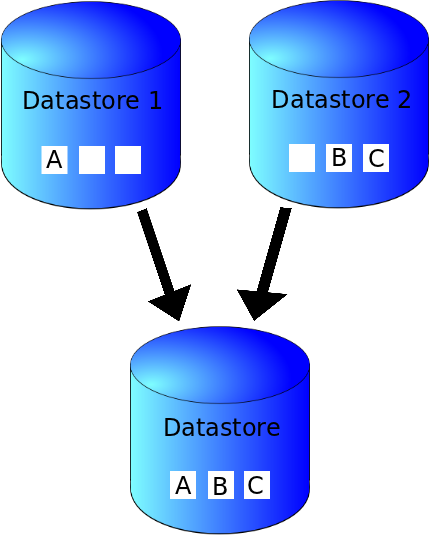
\includegraphics[scale=0.5]{project/images/data-sync}
  \caption{\textbf{IMAGE CAPTION}}
\end{figure}

\begin{lstlisting}
  PASTE YOUR CODE HERE
\end{lstlisting}
\newpage

 % adds the Project Design
%\chapter{Screenshots of Project}
\section{SECTION NAME}
\vspace{2cm}
\begin{figure}[H]
  \centering
    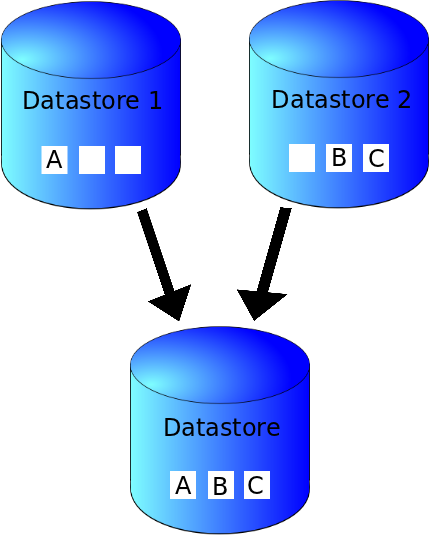
\includegraphics[height= 11cm, width=17cm]{project/images/data-sync}
\end{figure}
\newpage
\begin{figure}[H]
  \centering
    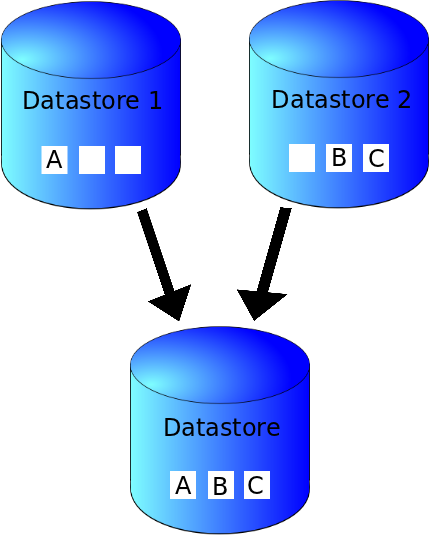
\includegraphics[height= 11cm, width=17cm]{project/images/data-sync}
\end{figure}
\vspace{1cm}
\begin{figure}[H]
  \centering
    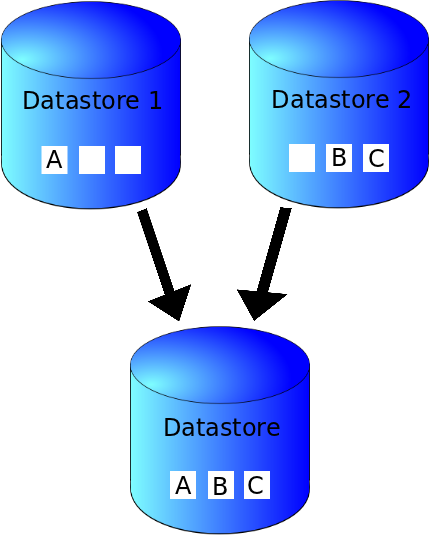
\includegraphics[height= 11cm, width=17cm]{project/images/data-sync}
\end{figure}
%\chapter{Conclusion and Future Scope}
\section{Conclusion}
\paragraph{}WRITE HERE.
\section{Future Scope}
\paragraph{}WRITE HERE.
\begin{itemize}
 \item ITEM 1
 \item ITEM 2
 \item ITEM 3
\end{itemize} % adds the Scheduling and Planning page
%\addcontentsline{toc}{chapter}{References}
\begin{thebibliography}{99}
\bibitem{WRITE A SHORT-NAME WITHOUT SPACE} \emph{NAME OF IEEE PAPER}; NAME OF AUTHORS
\bibitem{WRITE A SHORT-NAME WITHOUT SPACE} \url{http://EXAMPLE.com}
\end{thebibliography} % adds the References page

\bibliography{publication}
\bibliographystyle{plain}
\end{document}